\documentclass{article}

%% Denote paragraphs with vertical space rather than indenting (not critical)
\usepackage{parskip}

%% Support for URL in introductory text (not needed for main example)
\usepackage{url}

%% *** Enable TikZ ***
\usepackage{tikz}


\begin{document}

%% Introductory Text
Example 2.20 from the book\\
\emph{Unlocking LaTeX Graphics: A Concise Guide to Ti$k$Z/PGF and PGFPLOTS}.\\
For more information, visit \url{https://latex-graphics.com}.
\par\bigskip

%% *** START OF EXAMPLE CODE ***
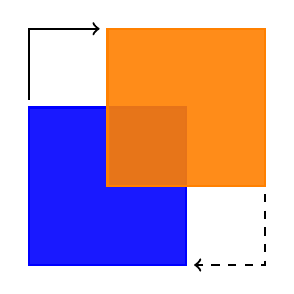
\begin{tikzpicture}[thick, fill opacity=0.9,
    arw/.style={->,shorten <=1mm, shorten >=1mm}]
  \filldraw[blue] (0,0) coordinate (BSW) rectangle ++(2,2) coordinate (BNE);
  \filldraw[orange] (1,1) coordinate (OSW) rectangle ++(2,2) coordinate (ONE);
  \draw[arw] (BSW |- BNE) -- (BSW |- ONE) -- (OSW |- ONE);
  \draw[arw,dashed] (ONE |- OSW) -- (ONE |- BSW) -- (BNE |- BSW);
\end{tikzpicture}
%% *** END OF EXAMPLE CODE ***

\end{document}
